\documentclass[../main2.tex]{subfiles}

\begin{document}
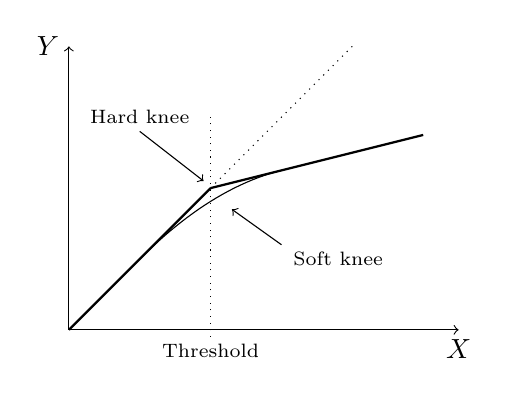
\begin{tikzpicture}[scale=0.9,baseline={(0,0)}]

% AXES
% horizontal axis
\draw[->] (0,0) -- (5.5,0) node[anchor=north] {$X$};
% vertical axis
\draw[->] (0,0) -- (0,4) node[anchor=east] {$Y$};

% GRAPH
% logy = logx
\draw[thick,domain=0:2] plot (\x,{\x});
% compression region
\draw[thick,domain=2:5] plot (\x,{\x + (1/4-1)*(\x-2)});
% soft knee
\draw[thin, domain=1:3] plot(\x, {\x + (1/4-1)*((\x-1)^2)/(4)});

\draw[dotted,domain=2:4] plot (\x,{\x});

% LABELS
% threshold
\draw[dotted] (2,-0.1) -- (2,3);
\draw(2,-0.3) node{{\scriptsize Threshold}};

% Knee label
\draw[->](1, 2.8) -- (1.9, 2.1);
\draw(1,3) node{{\scriptsize Hard knee}};

\draw[->](3, 1.2) -- (2.3, 1.7);
\draw(3.8, 1) node{{\scriptsize Soft knee}};

\end{tikzpicture}
\end{document}